\documentclass[a4paper, 12pt]{article}

%%% Работа с русским языком
\usepackage{cmap}					% поиск в PDF
\usepackage{mathtext} 				% русские буквы в формулах
\usepackage[T2A]{fontenc}			% кодировка
\usepackage[utf8]{inputenc}			% кодировка исходного текста
\usepackage[russian]{babel}	% локализация и переносы

%%% Дополнительная работа с математикой
\usepackage{amsmath,amsfonts,amssymb,amsthm,mathtools} % AMS
\usepackage{icomma} % "Умная" запятая: $0,2$ --- число, $0, 2$ --- перечисление

%% Номера формул
%\mathtoolsset{showonlyrefs=true} % Показывать номера только у тех формул, на которые есть \eqref{} в тексте.

%% Шрифты
\usepackage{euscript}	 % Шрифт Евклид
\usepackage{mathrsfs} % Красивый матшрифт

%% Поля
\usepackage[left=2cm,right=2cm,top=2cm,bottom=2cm,bindingoffset=0cm]{geometry}

%% Русские списки
\usepackage{enumitem}
\makeatletter
\AddEnumerateCounter{\asbuk}{\russian@alph}{щ}
\makeatother

%%% Работа с картинками
\usepackage{graphicx}  % Для вставки рисунков
\graphicspath{{images/}{images2/}}  % папки с картинками
\setlength\fboxsep{3pt} % Отступ рамки \fbox{} от рисунка
\setlength\fboxrule{1pt} % Толщина линий рамки \fbox{}
\usepackage{wrapfig} % Обтекание рисунков и таблиц текстом

%%% Работа с таблицами
\usepackage{array,tabularx,tabulary,booktabs} % Дополнительная работа с таблицами
\usepackage{longtable}  % Длинные таблицы
\usepackage{multirow} % Слияние строк в таблице

%% Красная строка
\setlength{\parindent}{2em}

%% Интервалы
\linespread{1}
\usepackage{multirow}

%% TikZ
\usepackage{tikz}
\usetikzlibrary{graphs,graphs.standard}

%% Верхний колонтитул
\usepackage{fancyhdr}
\pagestyle{fancy}

%% Перенос знаков в формулах (по Львовскому)
\newcommand*{\hm}[1]{#1\nobreak\discretionary{}
	{\hbox{$\mathsurround=0pt #1$}}{}}

%% Мои дополнения
\usepackage{float} %Добавляет возможность работы с командой [H] которая улучшает расположение на странице
\usepackage{gensymb} %Красивые градусы
\usepackage{graphicx}               % Импорт изображений
\usepackage{caption} % Пакет для подписей к рисункам, в частности, для работы caption*

% подключаем hyperref (для ссылок внутри  pdf)
\usepackage[unicode, pdftex]{hyperref}

%%% Теоремы
\theoremstyle{plain}                    % Это стиль по умолчанию, его можно не переопределять.
\renewcommand\qedsymbol{$\blacksquare$} % переопределение символа завершения доказательства

\newtheorem{theorem}{Теорема}[section] % Теорема (счетчик по секиям)
\newtheorem{proposition}{Утверждение}[section] % Утверждение (счетчик по секиям)
\newtheorem{definition}{Определение}[section] % Определение (счетчик по секиям)
\newtheorem{corollary}{Следствие}[theorem] % Следстиве (счетчик по теоремам)
\newtheorem{problem}{Задача}[section] % Задача (счетчик по секиям)
\newtheorem*{remark}{Примечание} % Примечание (можно переопределить, как Замечание)
\newtheorem{lemma}{Лемма}[section] % Лемма (счетчик по секиям)

\begin{document}
	\newcommand{\HRule}{\rule{\linewidth}{0.7mm}} % Defines a new command for the horizontal lines, change thickness here
	
	\begin{center}
		\large\textbf{Московский Физико-Технический Институт}\\ % Name of your university/college
		\large\textbf{(государственный университет)}
	
		\vfill
		
		\Large Лабораторная работа по курсу общей физики № *labnum*\\[0.5cm] % Preambule of your document title
		
		
		\HRule
		\\[0.4cm]
		{ \huge \bfseries *name of your labwork*}% Title of your document
		\\[0.4cm] 
		\HRule
		\\[0.5cm]
		
		\ \\
	\textbf{\large Автор:} \\	
	\large *your name* *groupname*\\ % Your name and something more, your group num for example
		\vfill
		\hspace*{-0.8 cm}
\includegraphics[width=100 pt]{frkt_logo}\\ % logo of your  company/university/college
		\large Долгопрудный, 2021 % location and year
	\end{center}

\newpage
\setcounter{page}{2}
\fancyfoot[c]{\thepage}
\fancyhead[L] {Работа № *labnum*} % some information in page header
\fancyhead[R]{}
	
	
	\section*{Аннотация}
	
	\subsection*{Цель и оборудование}
	
	\begin{enumerate}
		\item \textbf{Цель работы:} изучение дифракция света на синусоидальной акустической решётке и наблюдение фазовой решётки методом тёмного поля.
		
		\item \textbf{В работе используются:} оптическая скамья, осветитель, два длиннофокусных объектива, кювета с жидкостью, кварцевый излучатель с микрометрическим винтом, генератор ультрозвуковой частоты, линза, вертикальная нить на рейтере, микроскоп.		
	\end{enumerate}    
	
	\subsection*{Теоретическое введние}	
	
	В работе используются оптическая скамья, осветитель, два длиннофокусных объектива, кювета с жидкостью, кварцевый излучатель с микрометрическим винтом, генератор звуковой частоты, линза, горизонтальная нить на рейтере, микроскоп. 
	
	При прохождении ультразвуковой волны через жидкость в ней возникают периодические неоднородности коэффициента преломления, создается фазовая решетка, которую мы считаем неподвижной ввиду малости скорости звука относительно скорости света. Показатель
	преломления n изменяется по закону:
	
	\begin{equation}\label{}
	n = n_0 (1 + m \cos \Omega x)
	\end{equation}
	
	Здесь $ \Omega = 2 \pi / \Lambda $ --- волновое число для ультразвуковой волны, $ m $ --- глубина модуляции $ n $ $ (m \ll 1 $).
	
	Положим фазу $ \phi $ колебаний световой волны на передней стенке кюветы равной нулю, тогда на задней поверхности она равна:
	
	\begin{equation}\label{}
	\phi  = k n L = \phi_0 (1 + m \cos \Omega x)
	\end{equation}
	
	Здесь $ L $ --- толщина жидкости в кювете, $ k = 2 \pi / \lambda $ --- волновое число для света.
	
	После прохождения через кювету световое поле есть совокупность плоских волн, распространяющихся под углами $ \theta $, соответствующими максимумам в дифракции Фраунгофера:
	
	\begin{equation}\label{}	
	\Lambda \sin \theta_m = m \lambda
	\end{equation}
	
	Этот эффект проиллюстрирован на рисунке 1.
	\begin{figure}[H]
		\centering	
		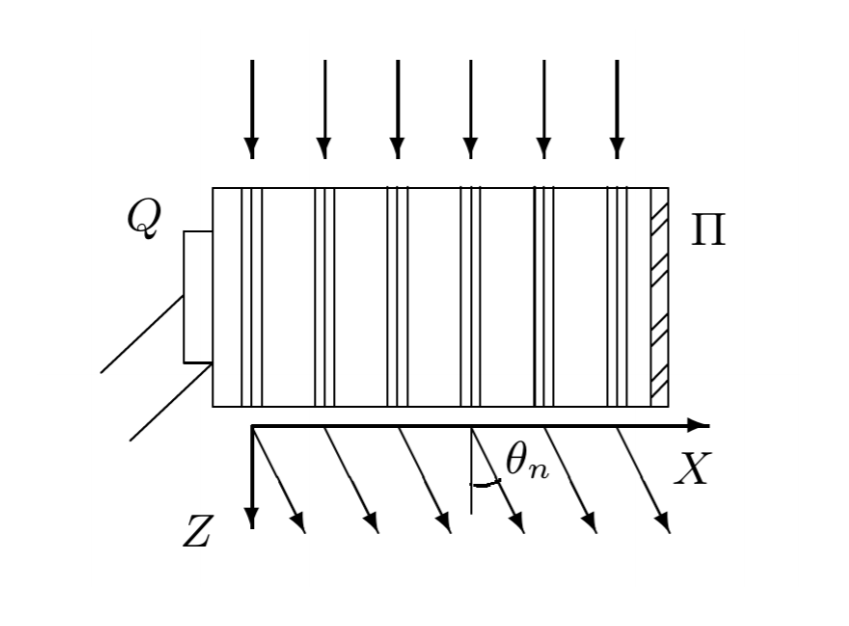
\includegraphics[scale = 0.3]{images/pic_1.png}
		\caption{Дифракция световых волн на акустической решетке}
		\label{diff}
	\end{figure}
	
	Зная положение дифракционных максимумов, по формуле (1) легко определить длину ультразвуковой волны, учитывая малость $ \theta $: $ \sin \theta \approx \theta \approx l_m /F  $, где $ l_m $ --- расстояние от нулевого до последнего видимого максимума, $ F $ --- фокусное расстояние линзы. Тогда получим:
	
	\begin{equation}\label{}
	\Lambda = m \lambda F/ l_m 
	\end{equation}
	Скорость ультразвуковых волн в жидкости, где $ \nu $ --- частота колебаний излучателя:
	
	\begin{equation}\label{}
	v = \Lambda \nu 
	\end{equation}
	
	\subsection*{Эксперементальная установка}
	
	\textbf{Схема установки. }Схема установки приведена на рисунке 2. Источник света Л через светофильтр Ф и конденсор К освещает вертикальную щель $ S $, находящуюся в фокусе объектива $ O_1 $. После объектива параллельный световой пучок проходит через кювету С перпендикулярно акустической решетке, и дифракционная картина собирается в фокальной плоскости объектива $ O_2 $ , наблюдается при помощи микроскопа М.
	
	Предварительную настройку установки произведем в соответствии с инструкцией с зеленым фильтром, далее в работе используется красный.
	
	\begin{figure}[H]
		\centering	
		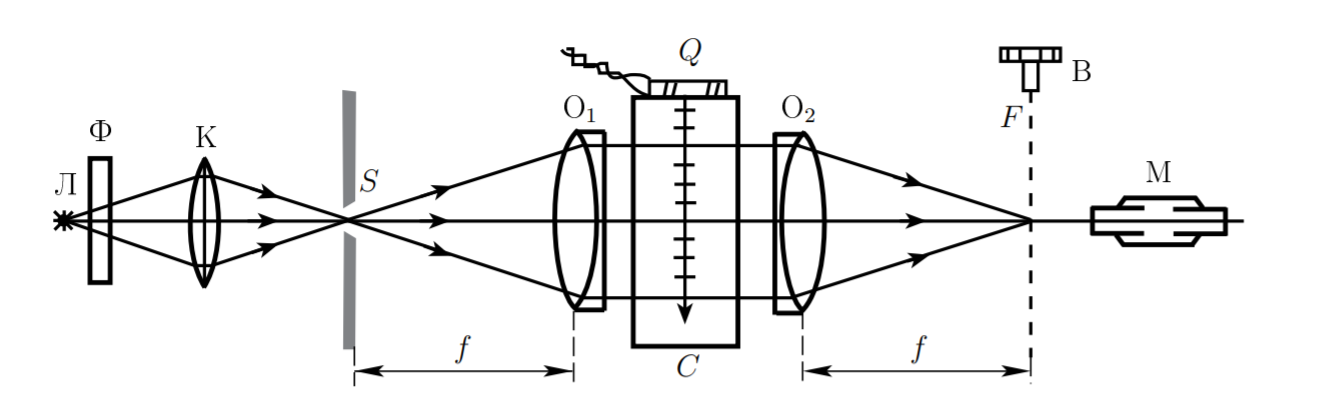
\includegraphics[scale=0.3]{images/pic_2.png}
		\caption{Схема для наблюдения дифракции на акустической решетке}
		\label{shema1}
	\end{figure}
	
	Параметры установки: фокусное расстояние объектива $F = 30 $ см, одно деление винта микроскопа составляет 20~мкм, полоса пропускания фильтра \mbox{$\lambda = 6400\pm 200$ Å}.
	
	Для определения скорости ультразвука методом темного поля будем использовать следующую установку.
	\begin{figure}[H]
		\centering	
		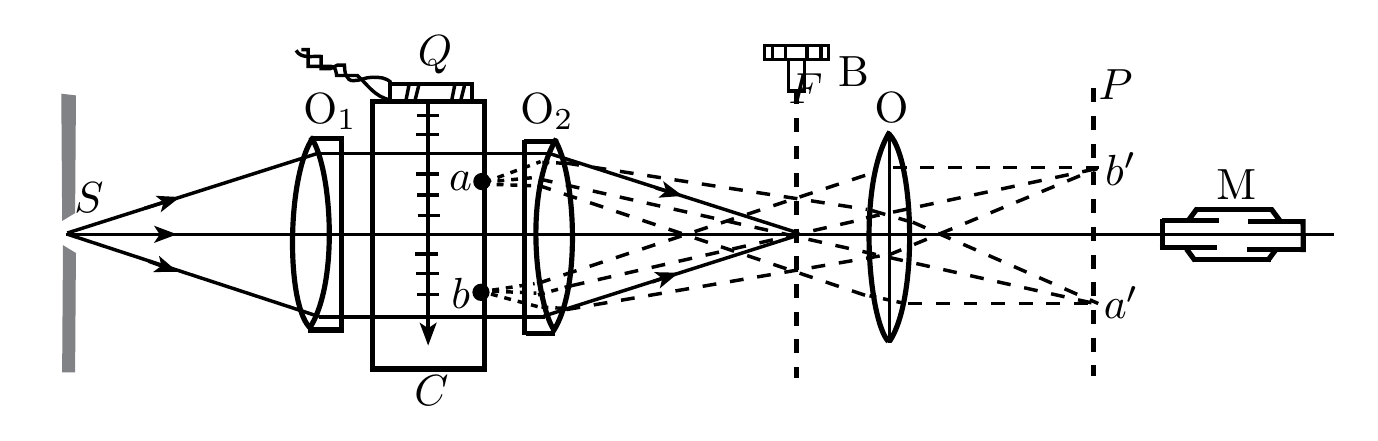
\includegraphics[scale=0.6]{pic_7.png}
		\caption{Схема для определения скорости ультразвука методом темного поля}
		\label{shema2}
	\end{figure}

	\section*{Ход работы}
	
	\subsection*{Определение скорости ультразвука по дифракционной картине}
	
	Проводить эксперимент будем с использованием установки рис \ref{shema1}. Запишем параметры установки.
	
	\begin{center}
		Фокусные расстояние объективов: $F_1 = F_2 = 30$ см\\
		Длина волны и полоса пропускания для зеленого света: $\lambda_{\text{зел}} = 546 ~ \pm ~ 495$ нм \\
		Длина волны и полоса пропускания для красного света: $\lambda_{\text{крас}} = 640 ~ \pm ~ 20$ нм \\
	\end{center}

	Исследуем изменение дифракционной картины в зеленом и красном свете. \textbf{Полученные выводы:} 
	
	\begin{enumerate}
		\item При уменьшении мощности УЗ число дифракционных полос уменьшается.
		\item При замене светофильтра с зеленого на красный качество дифракционной картины улучшается.
		\item При наблюдении дифракционной картины в немонохроматическом свете качество дифракционной картины ухудшается. Это связано с временной когерентностью.
	\end{enumerate}

	Измерим положение $x$ дифракционных максимумов на разных частотах, по полученным данным построим графики зависимости $x(n)$. 
	
	Экспериментальные данные приведены в таблицах \ref{tab:frequency1}, \ref{tab:frequency2}, \ref{tab:frequency3} и \ref{tab:frequency4}.
	
	\begin{table}[h!]
    \centering
    \begin{tabular}{|c|c|c|c|c|c|c|c|}
    \hline
    $n$      & -3   & -2   & -1   & 0 & 1   & 2   & 3   \\ \hline
    $x$, дел & -102 & -72  & -36  & 0 & 33  & 67  & 108 \\ \hline
    $x$, мкм & -408 & -288 & -144 & 0 & 132 & 268 & 432 \\ \hline
    \end{tabular}
    \caption{Положение максимумов при $f = 1.03678$ МГц}
    \label{tab:frequency1}
\end{table}
	
	\begin{figure}
		\centering
		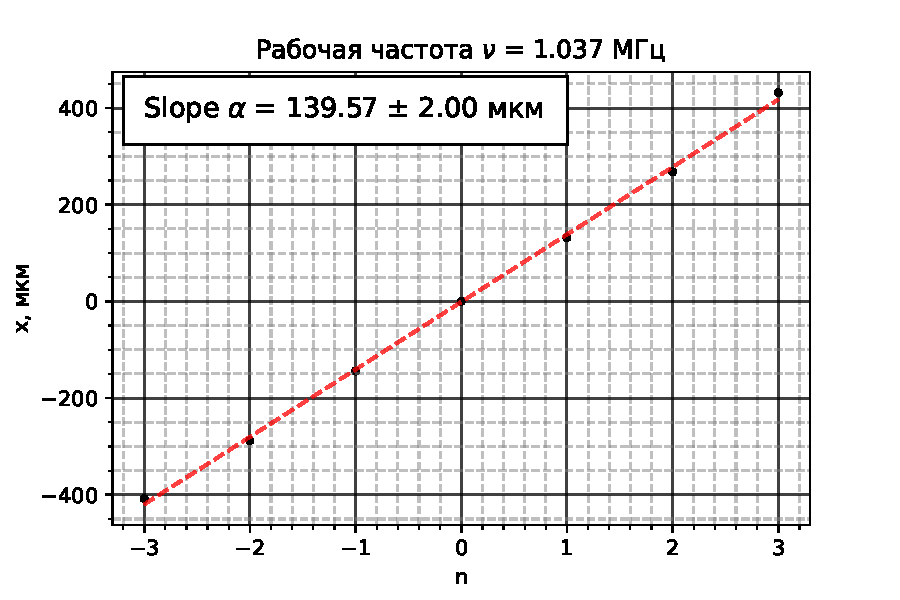
\includegraphics[scale=1]{./images/frequency1.ods.pdf}
		% \caption{text}
		\label{fig:frequency1}
	\end{figure}
	
	\begin{table}[h!]
    \centering
    \begin{tabular}{|c|c|c|c|c|c|c|c|}
    \hline
    $n$      & -3   & -2   & -1   & 0 & 1   & 2   & 3   \\ \hline
    $x$, дел & -104 & -72  & -36  & 0 & 35  & 70  & 110 \\ \hline
    $x$, мкм & -416 & -288 & -144 & 0 & 140 & 280 & 440 \\ \hline
    \end{tabular}
    \caption{Положение максимумов при $f = 1.07482$ МГц}
    \label{tab:frequency2}
\end{table}
	
	\begin{figure}
		\centering
		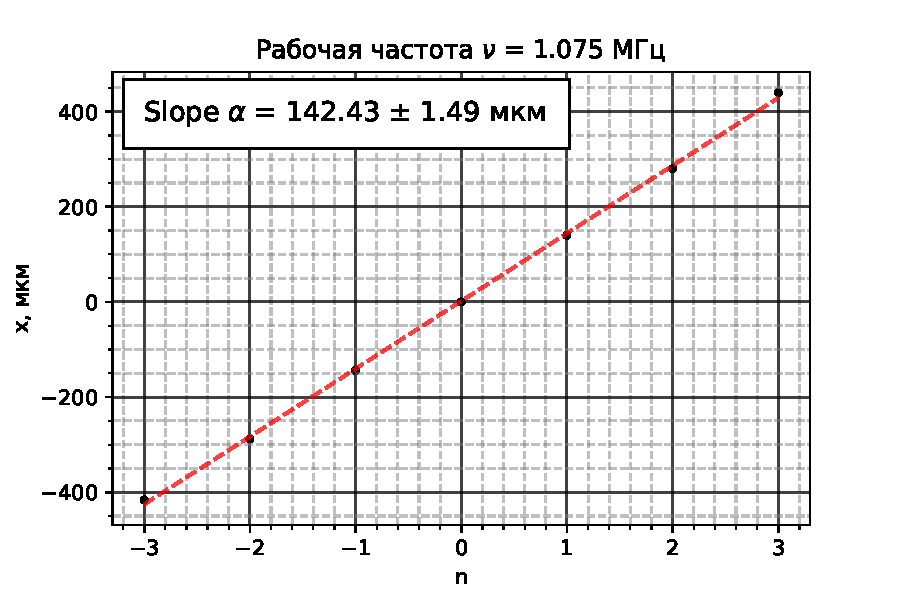
\includegraphics[scale=1]{./images/frequency2.ods.pdf}
		% \caption{text}
		\label{fig:frequency2}
	\end{figure}
	
	\begin{table}[h!]
    \centering
    \begin{tabular}{|c|c|c|c|c|c|c|c|}
    \hline
    $n$      & -3   & -2   & -1   & 0 & 1   & 2   & 3   \\ \hline
    $x$, дел & -107 & -74  & -36  & 0 & 37  & 72  & 111 \\ \hline
    $x$, мкм & -428 & -296 & -144 & 0 & 148 & 288 & 444 \\ \hline
    \end{tabular}
    \caption{Положение максимумов при $f = 1.10083$ МГц}
    \label{tab:frequency3}
\end{table}
	
	\begin{figure}
		\centering
		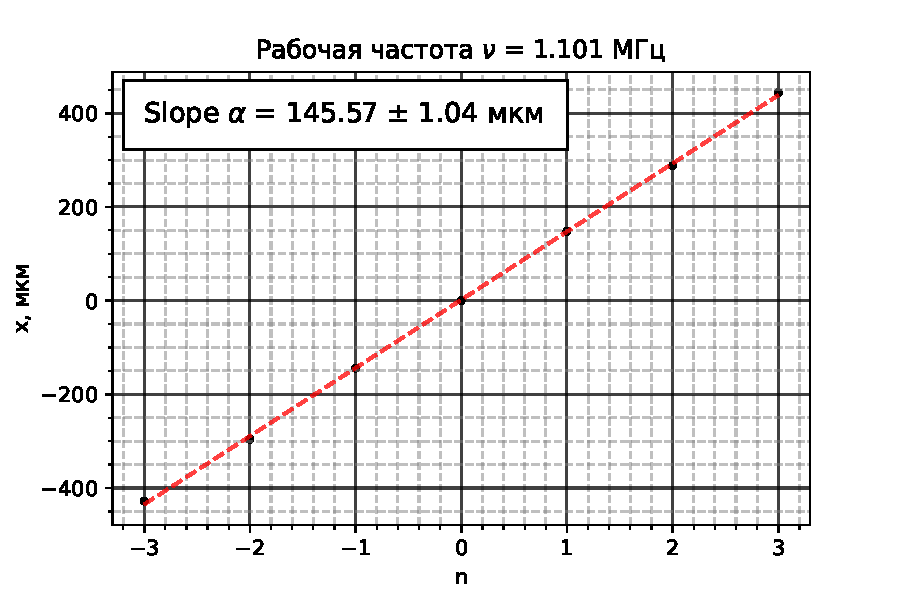
\includegraphics[scale=1]{./images/frequency3.ods.pdf}
		% \caption{text}
		\label{fig:frequency3}
	\end{figure}
	
	\begin{table}[h!]
    \centering
    \begin{tabular}{|c|c|c|c|c|c|c|c|}
    \hline
    $n$      & -3   & -2   & -1   & 0 & 1   & 2   & 3   \\ \hline
    $x$, дел & -120 & -74  & -31  & 0 & 39  & 80  & 121 \\ \hline
    $x$, мкм & -480 & -296 & -124 & 0 & 156 & 320 & 484 \\ \hline
    \end{tabular}
    \caption{Положение максимумов при $f = 1.22206$ МГц}
    \label{tab:frequency4}
\end{table}
	
	\begin{figure}
		\centering
		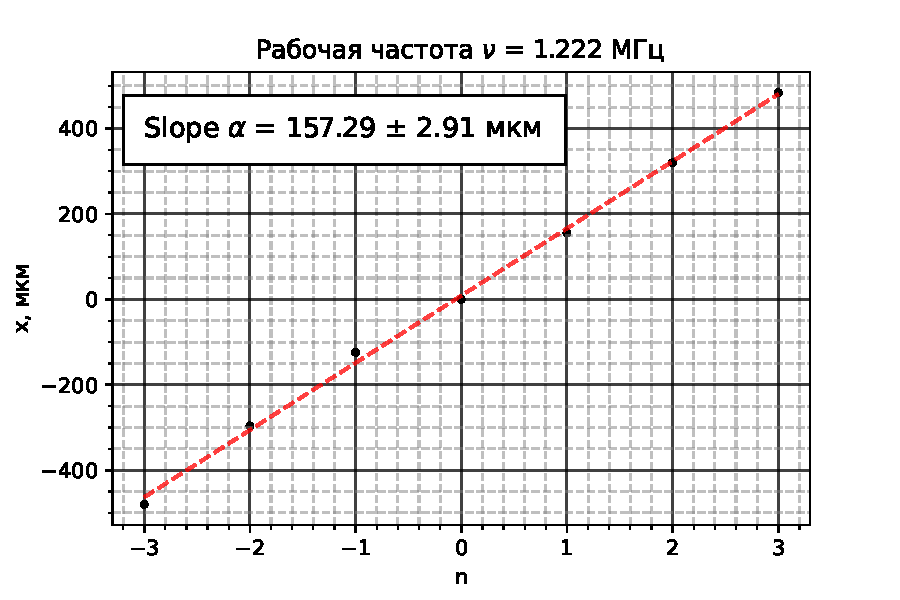
\includegraphics[scale=1]{./images/frequency4.ods.pdf}
		% \caption{text}
		\label{fig:frequency4}
	\end{figure}

	По наклону каждого графика можно определить среднее расстояние между двумя максимумами, а зная длину волны найдем длину ультразвуковой волны по формуле:
	
	\[ \alpha = \frac{l_m}{m} = f \frac{\lambda}{\Lambda} \]
	
	где $l_m$ -- среднее расстояние между максимумами, $\alpha$ -- наклон графика, $\Lambda$ -- длина УЗ волны. Зная величину $\Lambda$ можем вычислить скорость УЗ по формуле
	
	\[v = \Lambda \nu \]
	
	Расчет погрешностей
	
	\[ \frac{\sigma_{\Lambda}}{\Lambda} = \frac{\sigma_{\alpha}}{\alpha} \Rightarrow \sigma_{\Lambda} = \frac{\sigma_{\alpha}}{\alpha} \Lambda \]
	
	\[ \sigma_{v} = \sqrt{\varepsilon_{\Lambda}^2 + \varepsilon_{\nu}^2} v \]
	
	где $\nu$ -- частота УЗ. Результаты вычислений приведены в таблице \ref{tab:res}.
	
	\begin{table}[h!]
    \centering
    \begin{tabular}{|c|c|c|c|c|c|c|}
    \hline
    $f$, МГц     & $\alpha$, мкм  & $\sigma_{\alpha}$, мкм & $\Lambda$, мкм   & $\sigma_{\Lambda}$, мкм & $v$, м/с        & $\sigma_v$, м/с \\ \hline
    1,037        & 139,57         & 2,00                   & 1 375,65         & 19,71                   & 1 426,55        & 20,44           \\ \hline
    1,075        & 142,43         & 1,49                   & 1 348,03         & 14,10                   & 1 449,13        & 15,16           \\ \hline
    1,101        & 145,57         & 1,04                   & 1 318,95         & 9,42                    & 1 452,17        & 10,38           \\ \hline
    1,222        & 157,29         & 2,91                   & 1 220,68         & 22,58                   & 1 491,67        & 27,60           \\ \hline
    \end{tabular}
    \caption{Результаты вычислений}
    \label{tab:res}
\end{table}
	
	\subsection*{Определение скорости ультразвука методом темного поля}
	
	Для данного эксперимента будем использовать установку \ref{shema2}. Установим цену деления окулярной шкалы в условиях опыта.
	
	Получим изображение УЗ решетки, с помощью окулярной шкалы найдем расстояние между двумя удаленными минимумами и посчитаем количество полос между ними.
	
	Без применения метода темного поля звуковая решетка не наблюдается. Закроем нулевой максимум горизонтальной нитью. Таким образом, осевая составляющая фазово-модулированной волны поглощается, а боковые остаются без изменения. Получившееся поле: 
	
	\begin{equation}\label{}
	f(x) = \dfrac{im}{2} e^{i\Omega x} +  \dfrac{im}{2} e^{-i\Omega x} = im \cos \Omega x \te I(x) = m^2 \cos ^2 \Omega x = m^2 \dfrac{1 + \cos ^2 2 \Omega x}{2}
	\end{equation}
	
	Отсюда получаем, что расстояние между темными полосами есть $ \Lambda/2 $.
	
	Проведем измерение длины ультразвуковой волны, приняв ошибку равной цене деления окулярной шкалы.
	
	Формулы для расчета длины волны ультразвука $ \Lambda $ и скорости распространения $ v $ в воде:
	
	\begin{equation}\label{}
	\Lambda/2  = NC/(n - 1),  \qquad v = \nu\Lambda
	\end{equation}
	
	\begin{table}
		\centering
		\begin{tabular}{|c|c|c|c|c|c|c|c|c|}
			\hline
			$\nu$, Мгц & Количество делений $N$ & Количество темных полос $n$ & $\Lambda$, мм & $v$, м/с \\ \hline
			1,220 & 150 & 15 & 1,29 & 1570 \\ \hline
			1,259 & 150 & 16 & 1,20 & 1510 \\ \hline
			1,271 & 175 & 18 & 1,24 & 1570 \\ \hline
		\end{tabular}
	\end{table}

	\subsection*{Качественные наблюдения}
	
	Если последовательно закрывать нулевой, первый и второй максимумы дифракционной картины, то качество наблюдаемой УЗ решетки будет ухудшаться (см. рис \ref{1}, \ref{2}, \ref{3}).
	
	\begin{figure}
		\centering
		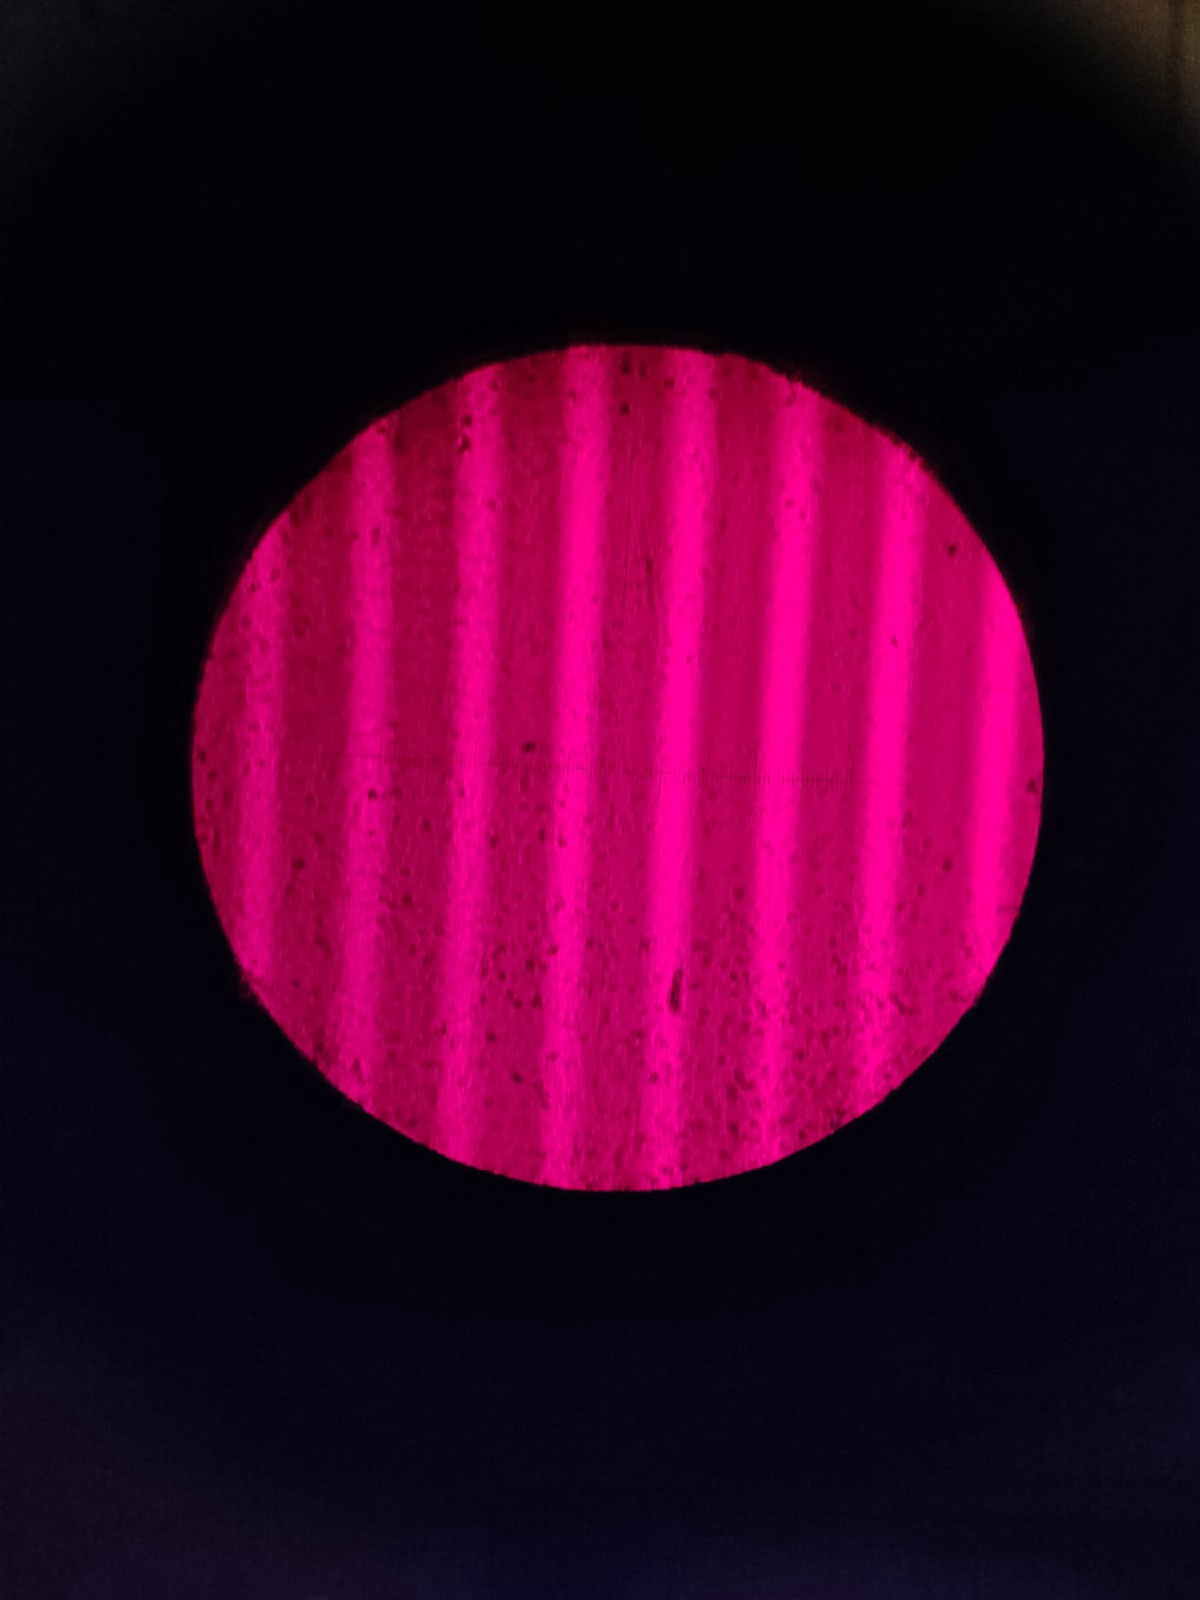
\includegraphics[width=0.5\linewidth]{./images/фазовая_решетка_закрыт_нулевой_максимум}
		\caption{фазовая решетка закрыт нулевой максимум}
		\label{1}
	\end{figure}

	\begin{figure}[h!]
		\begin{center}
			\begin{minipage}[h!]{0.48\linewidth}
				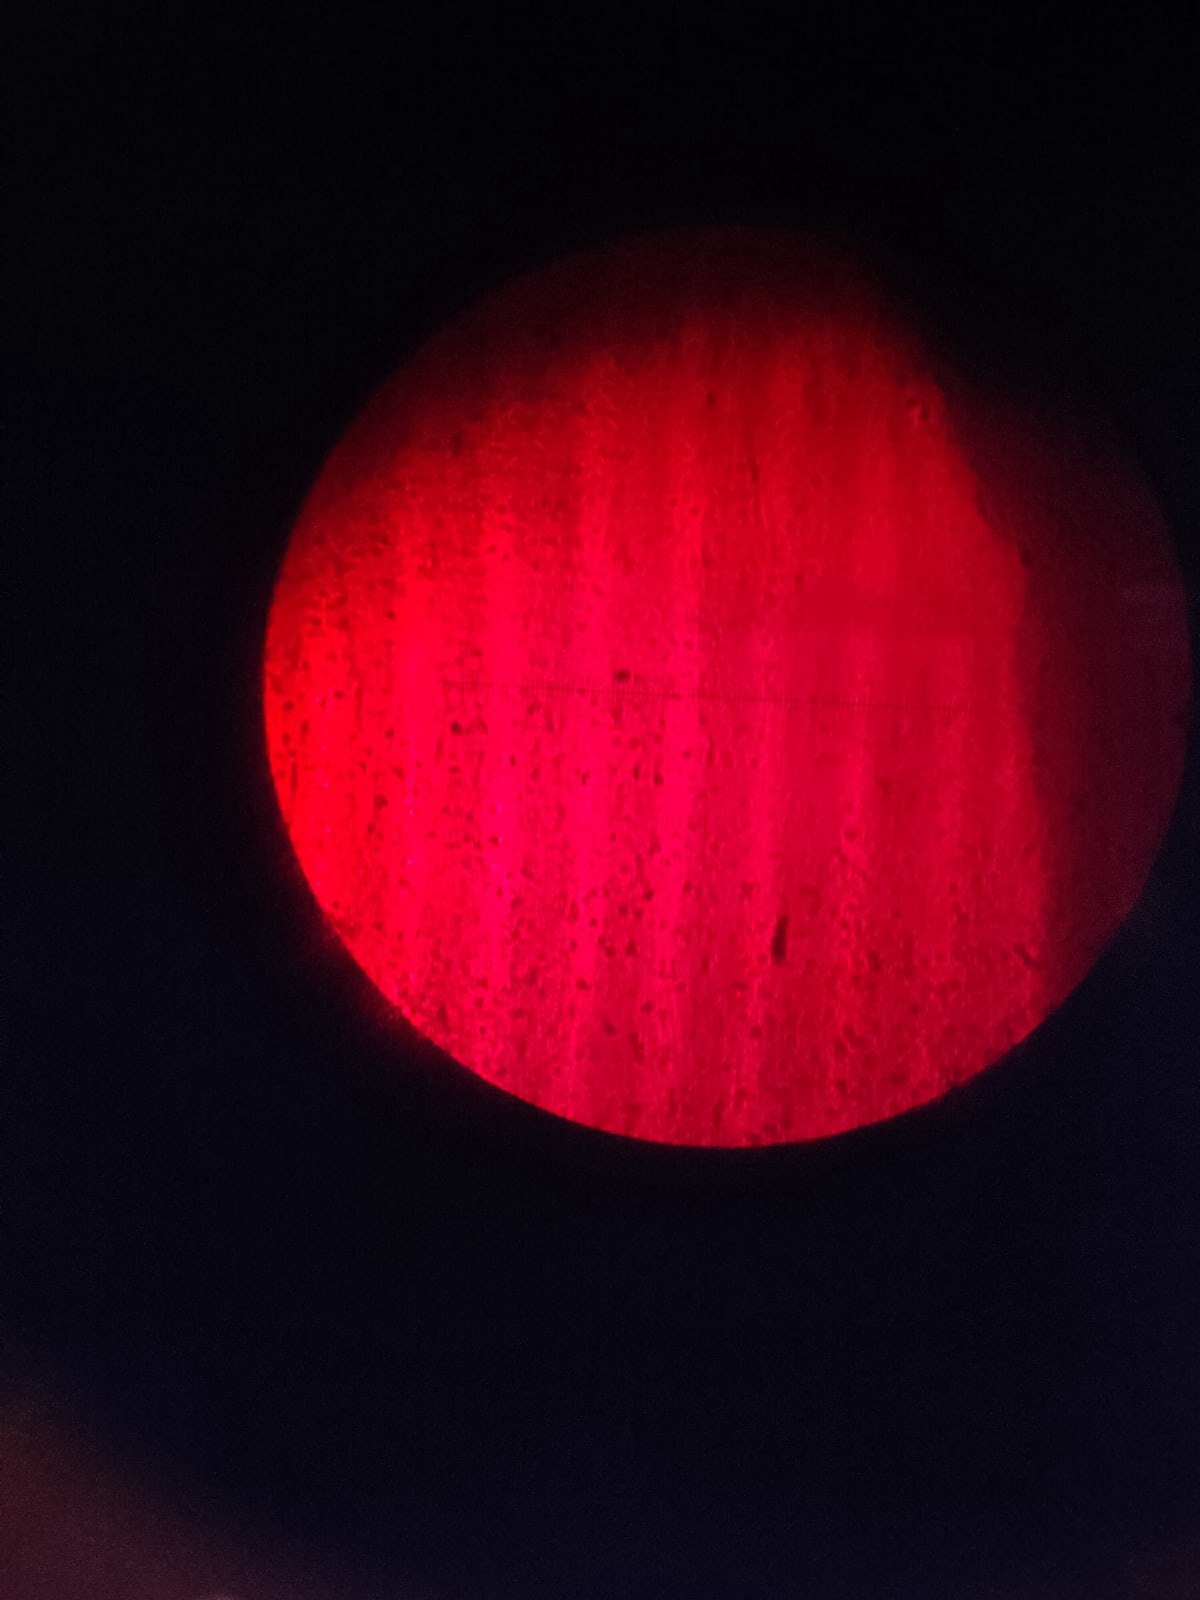
\includegraphics[width=1\linewidth]{./images/фазовая_решетка_закрыт_первый_максимум}
				\caption{фазовая решетка закрыт первый максимум}
				\label{2}
			\end{minipage}
			\hfill
			\begin{minipage}[h!]{0.48\linewidth}
				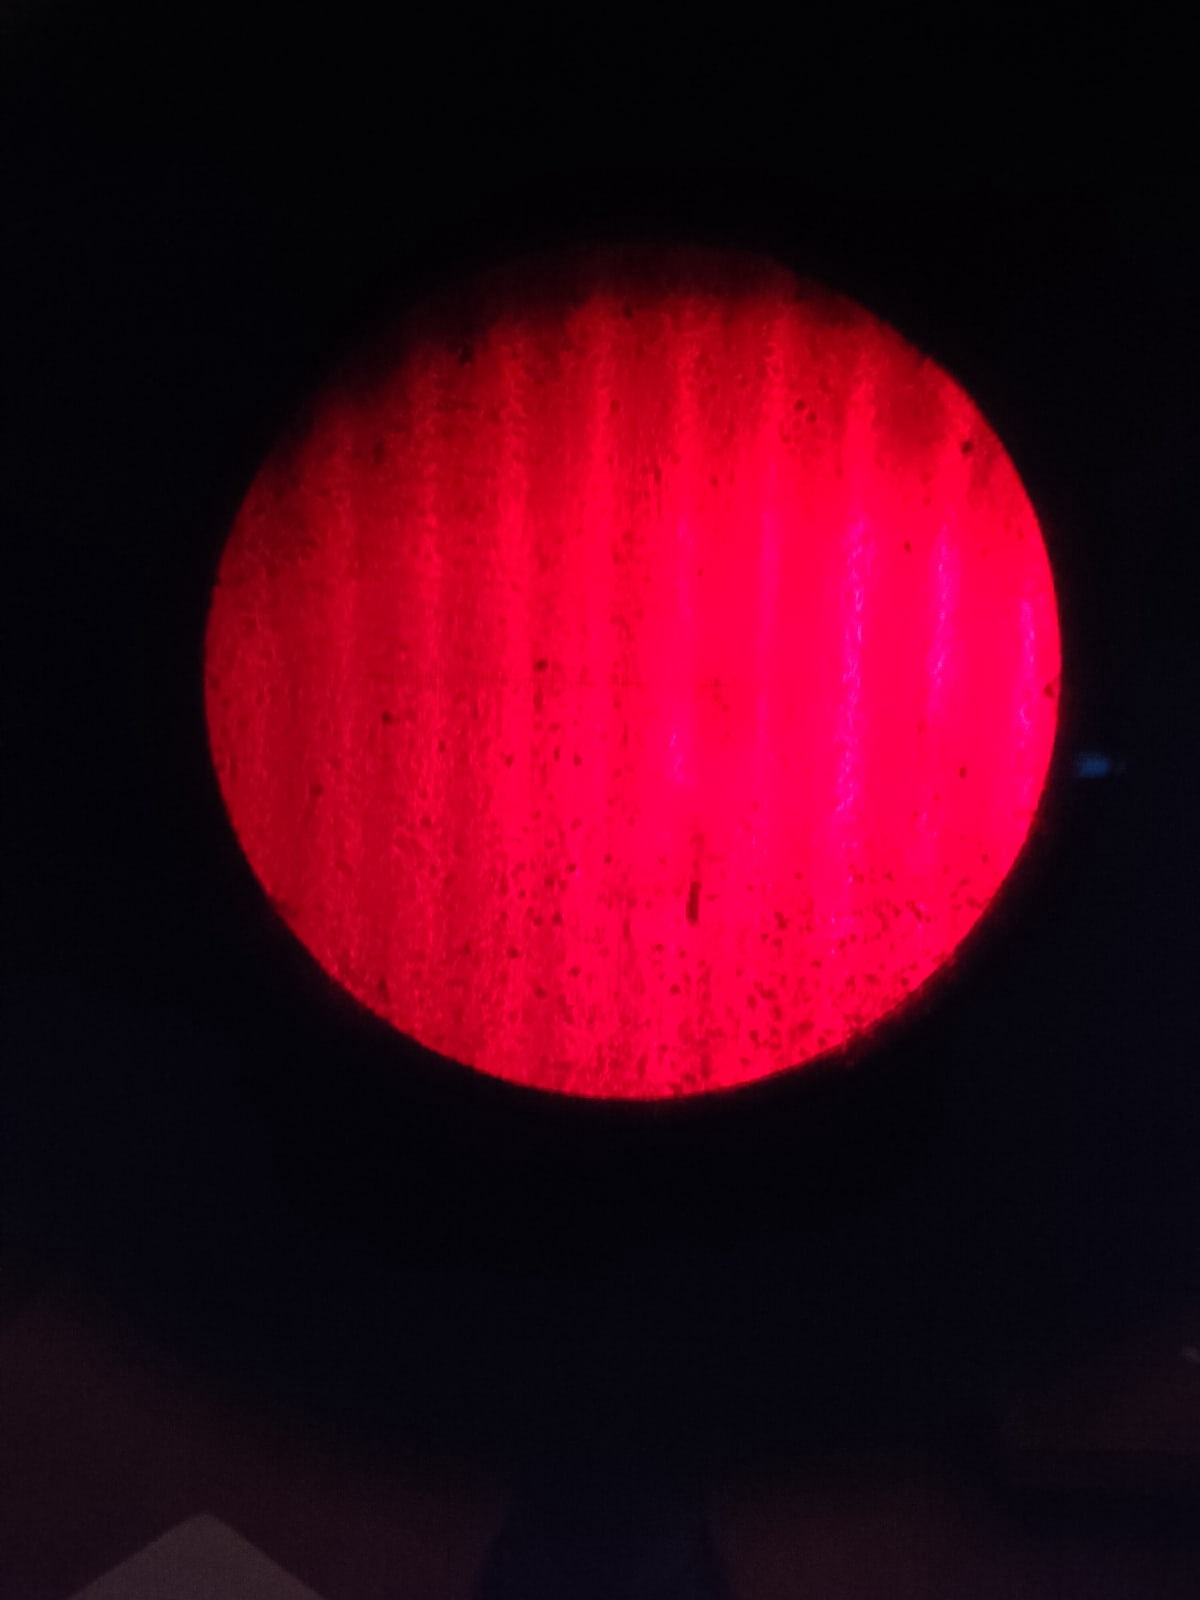
\includegraphics[width=1\linewidth]{./images/фазовая_решетка_закрыт_второй_максимум}
				\caption{фазовая решетка закрыт второй максимум}
				\label{3}
			\end{minipage}
		\end{center}
	\end{figure}

	\section{Вывод}
	
	В ходе проведения эксперимента мы измерили длину УЗ волны, а так же скорость УЗ. Пронаблюдали дифракцию на фазовой решетке, получили изображение фазовой решетки методом темного поля и сделали некоторые интересные качественные наблюдения (см. выше). 

\end{document}